\documentclass[fr]{../../../../../../eplexam}

\usepackage{../../../math-EPL1103-exam}
\usepackage[SIunits]{../../../../../../eplunits}

\hypertitle{Math\'ematique}{3}{FSAB}{1103}{2012}{Janvier}{All}
{Delhaye Benjamin\and Legat Beno\^it}
{Jean-François Remacle et Grégoire Winckelmans}

\paragraph{Resource utile}
\url{http://www.forum-epl.be/viewtopic.php?t=10154}

\section{}
On considère l'EDP suivante pour $u(x,t)$:
$$2\alpha xt\frac{\partial u}{\partial x} + \frac{\partial u}{\partial t} = \beta u.$$
On cherche la solution pour $- \infty < x < \infty$ et pour
$t \geq 0$. La condition initiale est $u(s,0) = u_0\frac{s}{L}$ avec $L$ une constante de longueur et $u_0$ une constante ayant les mêmes unités que $u$.
\begin{enumerate}
\item Quelles sont les dimensions des constantes $\alpha$ et $\beta$ ?
\item Obtenez le réseau des caractéristiques: équation et dessin (propre, avec axes adimensionnels et chiffrés !) dans la partie supérieure du plan (ie, pour $t \geq0$)
\item Obtenez explicitement expression pour $u(x,t)$
\end{enumerate}

\begin{solution}
  \begin{enumerate}
    \item
      Supposons que $t$ soit exprimé en [\second], $x$ en [\meter] et $u$ en [$\gamma$]. Les dimension de $\alpha$ et $\beta$ sont respectivement $[\frac{1}{\second^2}]$ et $[\frac{1}{\second}]$. En effet, nous obtenons alors
      $[\frac{\meter\cdot \second \cdot \gamma}{\meter\cdot \second^2}] + [\frac{\gamma}{\second}] = [\frac{\gamma}{\second}]$.\\

    \item
      Les caractéristiques s'obtiennent grâce à l'équation :
      $$\dif x = 2\alpha xt\dif t.$$
      Ou encore,
      $$\int_s^x \frac{\dif x'}{x}=2\alpha \int_0^t t\dif t'.$$
      Ce qui donne,
      $$\ln\left(\frac{x}{s}\right) = \alpha t^2.$$
      Finalement,
      $$x=se^{\alpha t^2}$$
      comme illustré par la figure~\ref{fig:cara}, autrement dit
      $$s=xe^{-\alpha t^2}.$$
      \begin{solfig}{cara}{Caractéristiques et $\Gamma\equiv t = 0$.}
        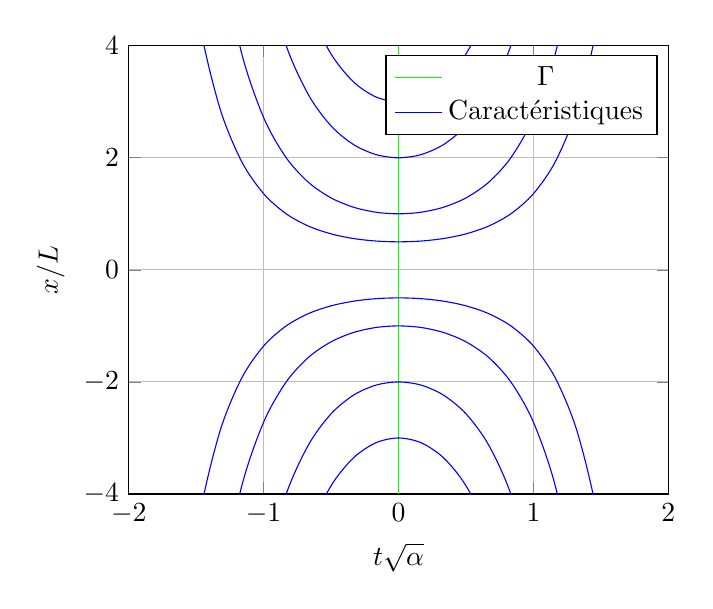
\begin{tikzpicture}
          \begin{axis}[xmin=-2,xmax=2,ymin=-4,ymax=4,
              xlabel = {$t\sqrt{\alpha}$},
            ylabel = {$x/L$}, grid]
            \addplot[green,smooth] plot coordinates {(0,-4) (0,4)};
            \addlegendentry{$\Gamma$};
            \addplot[blue,smooth,domain=-2:2]{-3*exp(x^2)};
            \addplot[blue,smooth,domain=-2:2]{-2*exp(x^2)};
            \addplot[blue,smooth,domain=-2:2]{-exp(x^2)};
            \addplot[blue,smooth,domain=-2:2]{-0.5*exp(x^2)};
            \addlegendentry{Caractéristiques};
            \addplot[blue,smooth,domain=-2:2]{0.5*exp(x^2)};
            \addplot[blue,smooth,domain=-2:2]{exp(x^2)};
            \addplot[blue,smooth,domain=-2:2]{2*exp(x^2)};
            \addplot[blue,smooth,domain=-2:2]{3*exp(x^2)};
          \end{axis}
        \end{tikzpicture}
      \end{solfig}

    \item
      Nous avons le choix entre deux équations qui nous mènent au même résultat :
      $$2\alpha xt \dif u = \beta u \dif x \text{\hspace{2cm}ou\hspace{2cm}} \dif u = \beta u \dif t.$$
      Nous prendrons ici la deuxième :
      $$\int_{u(s,0)}^{u(x,y)}\frac{\dif u'}{u} = \beta\int_0^t \dif t'.$$
      En développant les intégrales,
      \begin{align*}
        u(x,y) & = u(s,0)e^{\beta t} & \text{avec } u(s,0) = \frac{u_0}{L}xe^{-\alpha t^2}.
      \end{align*}
      Finalement,
      $$ u(x,y) = \frac{u_0x}{L}e^{\beta t-\alpha t^2}.$$
  \end{enumerate}
\end{solution}

\section{}
On considère l'EDP de Laplace pour $u(r,\theta)$ :
$$\nabla ^2u = \frac{\partial^2u}{\partial r^2} +\frac{1}{r} \frac{\partial u}{\partial r} + \frac{1}{r^2}\frac{\partial^2u}{\partial \theta^2} = 0  $$ dans un demi-cercle de rayon $a$. Sur le pourtour du demi-cercle, on impose que $\frac{\partial u}{\partial n} = g(\theta)$. Sur le diamètre du demi-cercle, on impose que $\frac{\partial u}{\partial n} = 0$. On impose finalement $u = u_0$ en $r = 0$.
\begin{enumerate}
\item Faites un dessin du domaine dans le plan physique $(x,y)$ et dans le système $(r,\theta)$ et indiquez les conditions aux limites sur chaque bord.
\item Obtenez par la méthode de séparation des variables, la solution sous forme d'un développement en série. Écrivez clairement les intégrales à effectuer pour obtenir les coefficients du développement.
\end{enumerate}

\begin{solution}
  \begin{enumerate}
    \item
      $n$ est la normale, au bords du demi-cercle, $n$ est le long de $r$ et au bord du diamètre, $n$ est le long de $\theta$ donc
      nous pouvons résumer les conditions de la sorte:
      \begin{enumerate}
        \item $\frac{\partial u}{\partial r}(a,\theta) = g(\theta)$;
        \item $\frac{\partial u}{\partial \theta}(r,0) = 0$;
        \item $\frac{\partial u}{\partial \theta}(r,\pi) = 0$;
        \item $u(0,\theta) = u_0 $.
      \end{enumerate}
    \item
      Il y a 2 conditions non-homogènes, on va donc devoir distinguer 2 cas.
      Par superposition, on aura une solution qui est la somme des deux si il y a une solution dans chaque cas.
      Dans chaque cas, on prendra la sommes des solutions pour chaque mode ayant une solution avant d'attaquer la solution non-homogène.

      Posons la séparation de variables suivante:
      $$u(r,\theta) = \Theta (\theta) \cdot R(r)$$
      En injectant dans l'EDP de l'énoncé on obtient:
      \begin{align*}
        -\frac{r^2R''+rR'}{R} & = \frac{\Theta ''}{\Theta} =  \pm k^2 \text{ ou } 0
      \end{align*}
      en posant $k > 0$ sans perte de généralité (vu qu'il est au carré).
      \begin{description}
        \item[Cas $u_0 = 0$]
          Commençons par faire les 3 modes
          \begin{description}
            \item[Mode $+k^2$]
              On commence on $\Theta$ car c'est lui qui a 2 conditions homogènes.

              \textbf{En $\Theta$ :}
              $$\Theta '' - k^2 \Theta = 0$$
              La solution générale de cette équation est : $\Theta(\theta) = A \exp(k\theta) + B \exp(k\theta)$.\\
              En imposant les 2 conditions frontières, $A = B = 0$, il n'y a donc pas de mode $+k^2$.
            \item[Mode $-k^2$]
              \textbf{En $\Theta$ :}
              $$ \Theta '' + k^2 \Theta = 0$$
              La solution générale de cette équation est : $\Theta(\theta) = A \cos(k\theta) + B \sin(k\theta)$.
              On calcule
              \[ \Theta'(\theta) = -A\sin(k\theta) + B\cos(k\theta) \]
              $\Theta'(0)$ nous donne $B = 0$
              puis $\Theta'(\pi)$ nous donne $k_n = n$ avec $n = 1, 2, \ldots$.
              Donc,
              \begin{align*}
                \Theta_n(\theta) & = A_n\cos(n\theta) & \text{avec }n = 1,2,3,\ldots
              \end{align*}

              \textbf{En $R$ :}
              $$r^2R''+rR'-n^2R = 0.$$
              La solution générale de cette équation est:
              $R_n = C_nr^n+D_nr^{-n}$.
              La condition en $r = 0$ ($u(0,\theta) = u_0$) donne $C_n \cdot 0  + D_n \cdot \infty = 0$.
              On voit que $D_n$ doit valoir 0.
              En fait, comme nous avons une solution finie en $r = 0$,
              le terme $r^{-n}$ ne convient pas ici.
              Nous obtenons donc:
              \begin{align*}
                R_n(r) & = C_nr^n & \text{avec }n = 0,1,2,3,\ldots\text{ et } r \ne 0.
              \end{align*}
            \item[Mode $0$]
              \textbf{En $\Theta$ :}
              $$\Theta'' = 0$$
              donc $\Theta(\theta) = A\theta + B$.
              Avec les deux conditions frontières, on trouve $A = 0$.

              \textbf{En $R$ :}
              $$r^2R''+rR'= 0.$$
              A comme solution une constant $C$ également.
              Mais la condition en $r = 0$ impose que $C = 0$.
              Il n'y a donc que la solution triviale.
          \end{description}
          \textbf{En $u$ :}
          $$u_1(r,\theta) = \sum_{n=1}^{\infty} G_n\cos(n\theta)r^n.$$
          Calculons
          $$\frac{\partial u}{\partial r}(a,\theta) = \sum_{n=1}^{\infty}G_n n a^{n-1} \cos(n\theta) = g(\theta).$$
          Par l'orthogonalité des cosinus, nous trouvons
          $$G_n n a^{n-1}\frac{\pi}{2} = \int_0^{\pi}g(\theta) \cos(n\theta) d\theta.$$
          Finalement
          $$G_n = \frac{2\int_0^{\pi}g(\theta) \cos(n\theta) d\theta}{\pi n a^{n-1}}.$$
          Nous trouvons donc :
          $$u_1(r,\theta) = \frac{2}{\pi}\sum_{n=1}^{\infty} \frac{\int_0^{\pi}g(\theta) \cos(n\theta) d\theta \cos(n\theta)r^n}{ n a^{n-1}}.$$
        \item[Cas $g(\theta) = 0$]
          Commençons par faire les 3 modes
          \begin{description}
            \item[Mode $+k^2$]
              Pareil que l'autre cas, pas de solution.
            \item[Mode $-k^2$]
              \textbf{En $\Theta$ :}
              Pareil que l'autre cas,
              \begin{align*}
                \Theta_n(\theta) & = A_n\cos(n\theta) & \text{avec }n = 1,2,3,\ldots
              \end{align*}

              \textbf{En $R$ :}
              Comme pour l'autre cas, on a
              $R_n(r) = C_nr^n$.
              Mais la condition en $r = 0$ nous donne
              $C_n \cdot 0 = u_0$
              qui est impossible à respecter.
              Pas de mode $-k^2$ non plus donc.
            \item[Mode $0$]
              \textbf{En $\Theta$ :}
              Comme pour l'autre cas, $\Theta(\theta) = A$.

              \textbf{En $R$ :}
              Comme pour l'autre cas, $R(r) = C$.
              La condition homogène est
              $R'(a) = 0$ qui est ici respectée sans problème.
          \end{description}
          \textbf{En $u$ :}
          On a
          $$u_2(r,\theta) = AC$$
          qu'on peut rassembler en une constante $D$
          $$u_2(r,\theta) = D.$$
          Calculons
          $$u_2(0,\theta) = D = u_0.$$
          d'où $u_0 = D$
          Nous trouvons donc :
          $$u_1(r,\theta) = u_0.$$
      \end{description}
      Par superposition, on a
      $$u(r,\theta) = u_0 + \frac{2}{\pi}\sum_{n=1}^{\infty} \frac{\int_0^{\pi}g(\theta) \cos(n\theta) d\theta \cos(n\theta)r^n}{ n a^{n-1}}.$$
  \end{enumerate}
\end{solution}


\section{}
On définit la fonction $$w = \arccos z = \frac{\pi}{2}-\int_0^z\frac{\dif z'}{\sqrt{1-z'^2}} = \frac{1}{i}\log \left(z+\sqrt{z^2-1}\right)$$
\begin{enumerate}
\item Obtenez les points de branchement de $w$ (\textbf{Aide}: $z+\sqrt{z^2-1}$ ne s'annule jamais). Proposez également un choix de coupure(s). Pour la suite, on utilisera la coupure principale.
\item Vérifiez que la définition de $w$ est bien telle que $\cos w = z$.
\item Obtenez l'expression de $w$ pour $z$ purement imaginaire ($z = iy$) et avec $y\geq 0$.
\item Obtenez le développement en série de $w$ autour de $z_0$. (\textbf{Aide}: obtenez d'abord le développement de $\frac{dw}{\dif z}$). Quel est le rayon de convergence de la série ?
\end{enumerate}
\rappelscomplexesbase
On a aussi, pour $|Z| < 1$, que
$\frac{1}{\sqrt{1-z}} = 1 + \frac{1}{2}z + \frac{1\cdot 3}{2 \cdot 4}z^2 + \frac{1 \cdot 3 \cdot 5}{2 \cdot 4 \cdot 6}z^3 + \ldots$

\begin{solution}
  \begin{enumerate}
    \item
      Nous pouvons décomposer $w$ est plusieurs fonctions de la façon suivante. Posons :
      \begin{enumerate}
        \item $h(z_1) = z_1^2-1$
        \item $g(z_2) = \sqrt{z_2}$
        \item $k(z_3) = \log(z_3)$
      \end{enumerate}
      Nous trouvons donc que $w = k(z+g(h(z)))$. \\
      Intéressons-nous tout d'abord à $h(z)$. Il s'agit d'un polynôme. $h(z)$ est donc continue et dérivable sur $C$ ($h$ est holomorphe). Elle ne présente donc pas de point de branchement, et donc pas de coupure. \\

      Intéressons-nous ensuite à $g(z)$. Il s'agit d'une fonction à exposant fractionnaire, qui est donc multiforme. Les points de branchement potentiels sont les points annulant l'argument de la fonction. Nous avons $g(z^2-1) = \sqrt{z^2-1}$. Nous avons donc 2 candidats : $z = -1$ et $z = 1$. Vérifions s'il s'agit bien de points de branchement : \\
      Posons \\
      $z-1 = r_0e^{i\theta_0 + 2n\pi}$ et\\
      $z+1 = r_1e^{i\theta_1 + 2m\pi}$.\\
      Nous trouvons : $g(z^2-1) = \sqrt{r_0r_1} e^{i\frac{\theta_0 + \theta_1}{2}+ (m+n)\pi}$ avec $\arg(g) = \frac{\theta_0 + \theta_1}{2}+ (m+n)\pi$.\\
      Pour $n = 0$ et $m = 0$, $g(z^2-1) = \sqrt{r_0r_1} e^{i\frac{\theta_0 + \theta_1}{2}}$.\\
      Pour $n = 1$ et $m = 0$ ou $n = 0$ et $m = 1$, $g(z^2-1) = \sqrt{r_0r_1} e^{i\frac{\theta_0 + \theta_1}{2}+\pi}$.\\
      Pour $n = 2$ et $m = 0$ ou $n = 1$ et $m = 1$ ou $n = 0$ et $m = 2$, $g(z^2-1) = \sqrt{r_0r_1} e^{i\frac{\theta_0 + \theta_1}{2}+ 2\pi} = \sqrt{r_0r_1} e^{i\frac{\theta_0 + \theta_1}{2}}$.\\

      Nous avons donc deux branches, et donc 2 points de branchement $z = -1$ et $z = 1$. Nous devons maintenant définir les deux coupures. Nous choisissons :
      $$\frac{-3\pi}{2} \leq \theta_0 \leq \frac{\pi}{2}$$
      $$\frac{-\pi}{2} \leq \theta_1 \leq \frac{3\pi}{2}.$$
      Ce qui nous permet de retomber sur le cas canonique :
      $$-\pi \leq \Arg(g) \leq \pi.$$
      Intéressons nous finalement à $k(z)$. La fonction $\log$ est multiforme. Mais comme ``$z+\sqrt{z^2-1}\neq 0$'', nous n'avons pas de nouveau candidat. \\

    \item
      Nous devons prouver que $\cos w = z$. Nous savons que :
      \begin{align*}
        \cos w :&= \frac{1}{2}(e^{iw}+e^{-iw})\\
                & = \frac{1}{2} \left( z+\sqrt{z^2-1}+\frac{1}{z+\sqrt{z^2-1}}\right)\\
                & = \frac{1}{2} \left(\frac{z^2+2z\sqrt{z^2-1}+z^2}{z+\sqrt{z^2-1}}\right)\\
                & = z.
      \end{align*}

    \item
      Posons $z=iy$ avec $y\geq 0$. Nous avons :
      \begin{align*}
        w &= \frac{1}{i}\log\left(iy+\sqrt{-y^2-1}\right)\\
          &= \frac{1}{i}\log\left(i(y+\sqrt{y^2+1})\right)\\
          &= \frac{1}{i}\left(\ln\left\vert i(y+\sqrt{y^2+1})\right\vert + i \arg\left(i(y+\sqrt{y^2+1})\right)\right)\\
          &= \frac{1}{i}\left(\ln\left(y+\sqrt{y^2+1}\right)+i\left(\frac{\pi}{2}+2n\pi\right)\right)\\
          &= \frac{\pi}{2} - i \ln\left(y+\sqrt{y^2+1}\right) +2n\pi.
      \end{align*}

    \item
      Commençons par calculer (grâce à l'aide de l'énoncé) :
      $$\frac{1}{\sqrt{1-z^2}} = 1 +\frac{1}{2}z^2 + \frac{1\cdot 3}{2\cdot 4}z^4 + \frac{1\cdot 3\cdot 5}{2\cdot 4\cdot 6}z^6+\ldots$$
      Nous trouvons donc,
      \begin{align*}
        w &= \arccos z \\
          & = \frac{\pi}{2}-\int_0^z\frac{\dif z'}{\sqrt{1-z'^2}}\\
          &= \frac{\pi}{2}-\int_0^z 1 +\frac{1}{2}z^2 + \frac{1\cdot 3}{2\cdot 4}z^4 + \frac{1\cdot 3\cdot 5}{2\cdot 4\cdot 6}z^6+\ldots \ \dif z\\
          &= \frac{\pi}{2}-\left[z +\frac{1}{2\cdot 3}z^3 + \frac{1\cdot 3}{2\cdot 4\cdot 5}z^5 + \frac{1\cdot 3\cdot 5}{2\cdot 4\cdot 6\cdot 7}z^7+\ldots\right]_0^z \\
          &= \frac{\pi}{2}- z -\frac{1}{2\cdot 3}z^3 - \frac{1\cdot 3}{2\cdot 4\cdot 5}z^5 - \frac{1\cdot 3\cdot 5}{2\cdot 4\cdot 6\cdot 7}z^7 - \ldots
      \end{align*}
      Le rayon de convergence est de 1 (= écart entre le point à évoluer, ici $z = 0$, et la première singularité, ici $z = 1$ et $z = -1$).
  \end{enumerate}
\end{solution}

\section{}
Calculez l'intégrale suivante : $$\int_0^\infty\frac{\sqrt[3]{x}}{x^2+1}\dif x$$
Pour rappel, $\cos\frac{\pi}{6} = \frac{\sqrt{3}}{2}$ et $\cos\frac{\pi}{3} = \frac{1}{2}$.

\begin{solution}
\emph{La résolution de cet exercice ressemble
énormément à l'exercice 2.6 de l'APE 12.}

On peut le résoudre soit avec un pacman, soit avec un demi-cercle.
Optons pour le demi-cercle.
Commençons par définir la coupure du point de branchement $z = 0$ en dehors
du demi-cercle: $-\frac{\pi}{2} \leq \theta < \frac{3\pi}{2}$.
On aurait choisit $0\leq \theta < 2\pi$ pour pacman.
On a donc une petite encoche en 0.
Son intégrale tend vers 0 par le troisième lemme de Jordan,
en effet, pour $|z| \to 0$, $\frac{z^{4/3}}{z^2 + 1}\to 0$.

L'intégrale du demi-cercle tend vers 0 par le premier lemme de Jordan,
en effet, pour $|z| \to \infty$, $\frac{z^{4/3}}{z^2 + 1}\to 0$.

$-i$ est en dehors du demi-disque encoché donc il n'y a que $i$ comme
pôle. Son résidu vaut
$$\res((z-i)\cdot f, i) = \frac{i^{1/3}}{i + i}
= \frac{\exp(i\pi/6)}{2i} = \frac{\sqrt{3} + i}{4i}.$$
On a donc
$$\lim_{\epsilon\to 0}\int_{-\infty}^{-\epsilon}f(z)\dif z
+ \int_{\epsilon}^\infty f(z)\dif z
= 2\pi i \frac{\sqrt{3} + i}{4i} = \pi \frac{\sqrt{3} + i}{2}.$$

On peut transformer la première intégrale en
$$-\int_{-\epsilon}^{-\infty}\frac{z^{1/3}}{z^2 + 1}\dif z$$
en posant $z = -w$ avec $w \in \mathbb{R}^+$, on a
\begin{align*}
  -\int_{z=-\epsilon}^{z=-\infty}\frac{(-w)^{1/3}}{(-w)^2 + 1}\dif z & =
  -\int_{-w=-\epsilon}^{-w=-\infty}\frac{(-1)^{1/3}w^{1/3}}{w^2 + 1}\dif (-w)\\
  & = \int_{w=\epsilon}^{w=\infty}
  \frac{\exp(i\frac{\pi}{3})w^{1/3}}{w^2 + 1}\dif w\\
  & = \frac{1 + i\sqrt{3}}{2}\int_{\epsilon}^{\infty}
  \frac{w^{1/3}}{w^2 + 1}\dif w
\end{align*}

Soit $I = \int_0^\infty f(x) \dif x$, on a donc
\begin{align*}
  \frac{1+i\sqrt{3}}{2}I + I & = \pi \frac{\sqrt{3} + i}{2}\\
  \frac{3+i\sqrt{3}}{2}I & = \pi \frac{\sqrt{3} + i}{2}\\
  3I+i\sqrt{3}I & = \pi \sqrt{3} + i\pi.
\end{align*}
Comme deux complexes sont égaux si et seulement si leurs parties
réelles et imaginaires sont égales, on a $3I = \pi\sqrt{3}$ et
$\sqrt{3}I = \pi$ qui donnent tous les deux
$$I = \pi\frac{\sqrt{3}}{3}.$$
\end{solution}

\end{document}
